\chapter{Godzilla and Kaijū: Nuclear Monsters and Tokusatsu}

\section{The original \emph{Gojira} (1954)}

\begin{center}
\begin{tabular}{ll}
\toprule
Title & \emph{Gojira} (\ja{ゴジラ}), Tōhō, released 3 November 1954 \\
Director & Honda Ishirō \\
Special effects & Tsuburaya Eiji \\
Producer & Tanaka Tomoyuki \\
Music & Ifukube Akira \\
Name & blend of \emph{gorira} (gorilla) and \emph{kujira} (whale) \\
\bottomrule
\end{tabular}
\end{center}

\subsection{Context: the Lucky Dragon incident}

On 1 March 1954 the United States tested a hydrogen bomb (``Castle Bravo'') at Bikini Atoll.
The fallout fell on the Japanese tuna boat \textbf{Daigo Fukuryū Maru} (\ja{第五福竜丸},
``Lucky Dragon No.\ 5''). All 23 crew suffered radiation sickness; the radio operator Kuboyama
Aikichi died in September. Contaminated tuna caused a national panic and led to a mass
petition movement against nuclear weapons. \emph{Gojira} opens with a fishing boat engulfed
by a flash of light at sea: every Japanese viewer in 1954 understood the reference.

\subsection{Plot}

\begin{enumerate}
  \item Ships vanish near Odo Island. Islanders speak of an ancient sea monster, Gojira,
        to whom girls were once sacrificed; a kagura-like ritual is performed.
  \item The paleontologist \textbf{Dr.\ Yamane} discovers radioactive footprints and a
        trilobite: Gojira is a prehistoric creature awakened and irradiated by H-bomb
        tests.
  \item Gojira attacks Tokyo twice, breathing radioactive fire. Scenes of flattened,
        burning neighbourhoods, a mother comforting her children (``we'll be with Daddy
        soon''), and overflowing hospitals with a Geiger counter clicking over a child
        recall the 1945 air raids and Hiroshima.
  \item The young scientist \textbf{Serizawa}, who lost an eye in the war, has invented the
        \textbf{Oxygen Destroyer}, a weapon more terrible than the H-bomb. He burns his
        notes, uses it once to kill Gojira in Tokyo Bay, and dies with the monster so that
        the weapon can never be reproduced.
  \item Dr.\ Yamane's final words: if nuclear testing continues, another Gojira may appear.
\end{enumerate}

\begin{important}[Readings of Godzilla (1954)]
\begin{itemize}
  \item \textbf{Nuclear allegory}: Godzilla is the bomb, a product of American testing
        visiting destruction on Japan for the third time (Hiroshima, Nagasaki, Bikini).
  \item \textbf{War memory}: the monster comes from the south Pacific (where many Japanese
        soldiers died) and walks the path of the 1945 firebombing; some critics (Kawamoto
        Saburō) read it as the ghost of the war dead returning to Tokyo.
  \item \textbf{Victim and perpetrator}: Godzilla is also a victim of the bomb. Serizawa's
        self-sacrifice echoes wartime sacrifice but is redirected to peace.
  \item \textbf{Science}: Yamane wants to study the monster rather than kill it; Serizawa
        fears what science can do. The film is ambivalent about science.
  \item \textbf{Religion}: Gojira is called a god on Odo Island; the ending resembles the
        pacification of an angry kami (Week 2) rather than simple destruction.
\end{itemize}
\end{important}

\begin{aside}
Compare the original Japanese film with the 1956 US version,
\emph{Godzilla, King of the Monsters!}, which cut most of the anti-nuclear material and
inserted Raymond Burr as an American reporter observing events. The comparison is a lesson
in how monsters change meaning when they cross borders.
\end{aside}

\section{Tokusatsu}

\begin{definition}[Tokusatsu]
\emph{Tokusatsu} (\ja{特撮}, ``special filming'') is the Japanese special-effects tradition
of live-action film and TV, using miniatures, suit actors (\emph{suitmation}) and practical
effects rather than stop-motion animation (contrast \emph{King Kong}, 1933, which inspired
Tanaka and Tsuburaya).
\end{definition}

\begin{itemize}
  \item Godzilla was played by a man in a heavy latex suit (Nakajima Haruo) walking through
        detailed 1:25 scale miniature sets of Tokyo.
  \item Tsuburaya Eiji had made wartime propaganda films (his miniature recreation of
        Pearl Harbor in \emph{The War at Sea from Hawaii to Malaya}, 1942, was so convincing
        that occupation authorities thought it was real footage).
  \item Tsuburaya Productions went on to create \textbf{Ultraman} (\ja{ウルトラマン}, 1966):
        a giant hero who fights a new kaijū every week. Later: the \emph{Kamen Rider}
        (1971) and \emph{Super Sentai} (1975; adapted as \emph{Power Rangers} in the US)
        franchises.
\end{itemize}

\section{The kaijū genre}

\begin{definition}[Kaijū]
\emph{Kaijū} (\ja{怪獣}, ``strange beast'') are giant monsters of film and TV. Godzilla
created a genre: the \emph{daikaijū eiga} (``giant monster movie''). Monsters wrestling
monsters, often destroying landmarks (Tokyo Tower, the Diet building), became a set formula.
\end{definition}

\begin{center}
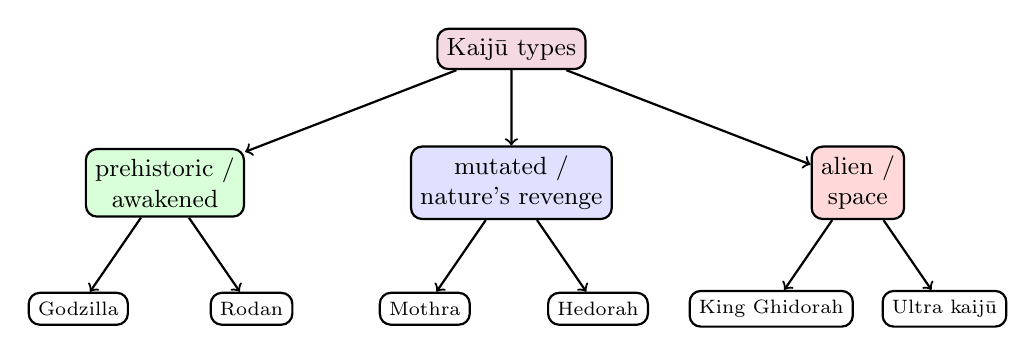
\begin{tikzpicture}[
    level 1/.style={sibling distance=4.4cm, level distance=1.7cm},
    level 2/.style={sibling distance=2.2cm, level distance=1.6cm},
    every node/.style={draw, thick, rounded corners, align=center, font=\small, fill=white},
    edge from parent/.style={draw, thick, ->}]
  \node[fill=purple!15] {Kaijū types}
    child { node[fill=green!15] {prehistoric /\\awakened}
      child { node[font=\scriptsize] {Godzilla} }
      child { node[font=\scriptsize] {Rodan} } }
    child { node[fill=blue!12] {mutated /\\nature's revenge}
      child { node[font=\scriptsize] {Mothra} }
      child { node[font=\scriptsize] {Hedorah} } }
    child { node[fill=red!15] {alien /\\space}
      child { node[font=\scriptsize] {King Ghidorah} }
      child { node[font=\scriptsize] {Ultra kaijū} } };
\end{tikzpicture}
\end{center}

\begin{center}
\begin{tabular}{llp{8.5cm}}
\toprule
Kaijū & Debut & Notes \\
\midrule
Rodan \ja{ラドン} & 1956 & giant pterosaur emerging from a coal mine \\
Mothra \ja{モスラ} & 1961 & giant moth, worshipped on Infant Island and summoned by twin fairies (the Shobijin) singing; a protector goddess; critique of exploitation of Pacific islanders \\
King Ghidorah \ja{キングギドラ} & 1964 & three-headed golden space dragon (compare Yamata no Orochi, Week 3) \\
Gamera \ja{ガメラ} & 1965 & Daiei studio's flying turtle; ``friend of all children'' \\
Hedorah \ja{ヘドラ} & 1971 & ``Smog Monster'' born of industrial pollution \\
\bottomrule
\end{tabular}
\end{center}

\section{Godzilla's eras}

\begin{center}
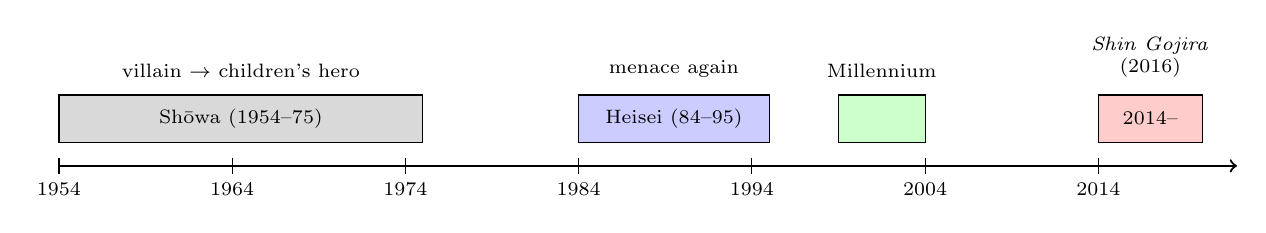
\begin{tikzpicture}[x=0.22cm, y=1cm, every node/.style={font=\scriptsize}]
  \draw[->, thick] (0,0) -- (68,0);
  \foreach \yr in {1954,1964,1974,1984,1994,2004,2014} {
    \pgfmathsetmacro{\x}{\yr-1954}
    \draw (\x,0.1) -- (\x,-0.1) node[below] {\yr};
  }
  \draw[fill=gray!30] (0,0.3) rectangle (21,0.9) node[midway] {Shōwa (1954--75)};
  \draw[fill=blue!20] (30,0.3) rectangle (41,0.9) node[midway] {Heisei (84--95)};
  \draw[fill=green!20] (45,0.3) rectangle (50,0.9); \node[above] at (47.5,1.0) {Millennium};
  \draw[fill=red!20] (60,0.3) rectangle (66,0.9) node[midway] {2014--};
  \node[above, align=center] at (10.5,1.0) {villain $\to$ children's hero};
  \node[above, align=center] at (35.5,1.0) {menace again};
  \node[above, align=center] at (63,1.0) {\emph{Shin Gojira}\\(2016)};
\end{tikzpicture}
\end{center}

\begin{itemize}
  \item \textbf{Shōwa series}: Godzilla quickly became a recurring, increasingly
        heroic figure who defends Japan against other monsters, with a son (Minilla) and
        comic scenes. The nuclear message faded as the audience became children.
  \item \textbf{Heisei series} (1984--1995): a darker reboot during Cold War tensions and
        the bubble era; Godzilla ``dies'' in a nuclear meltdown in 1995.
  \item \textbf{Hollywood}: TriStar's \emph{Godzilla} (1998) was disliked in Japan (Tōhō
        later renamed that creature ``Zilla''); Legendary's \emph{Godzilla} (2014) began a
        US ``MonsterVerse''.
  \item \textbf{\emph{Shin Gojira}} (\ja{シン・ゴジラ}, 2016), directed by Anno Hideaki
        (\emph{Evangelion}) and Higuchi Shinji: a new Godzilla evolves through grotesque
        stages while the government is paralysed by meetings and red tape. It was widely
        read as a response to the \textbf{2011 Tōhoku earthquake, tsunami and Fukushima
        nuclear disaster}: the monster is again radioactive, and the final freezing of
        Godzilla resembles the cooling of a reactor.
\end{itemize}

\section{Kaijū and yōkai compared}

\begin{center}
\begin{tabular}{p{3.2cm}p{4.8cm}p{4.8cm}}
\toprule
 & Yōkai & Kaijū \\
\midrule
Scale & human or smaller & enormous \\
Origin & folklore, local places & science fiction, nuclear tests, space \\
Medium & oral tale, scroll, manga & film and TV (tokusatsu) \\
Threat & individual (deception, possession) & collective (cities, nation) \\
Resolution & avoid, pacify, outwit & battle, sacrifice, coexistence \\
\bottomrule
\end{tabular}
\end{center}

Both share Cohen's category crisis, the logic of pacification rather than destruction, and
the long slide from terror to cute merchandise.

\begin{remark}
Tsutsui (\emph{Godzilla on My Mind}, 2004) argued that Godzilla's popularity reflects not
only fear but pleasure in destruction and in the craftsmanship of miniatures. Fear and
fun coexist, as with Edo yōkai.
\end{remark}

\section*{Summary}
\begin{itemize}
  \item \emph{Gojira} (1954, Honda Ishirō, Tsuburaya Eiji) responded to the Lucky Dragon
        incident and memories of 1945; Godzilla is both the bomb and its victim.
  \item Tokusatsu: suitmation and miniatures; Ultraman, Kamen Rider, Super Sentai.
  \item Kaijū genre: Rodan, Mothra, King Ghidorah, Gamera, Hedorah; monsters as nature's
        revenge.
  \item Godzilla shifts from menace to hero and back; \emph{Shin Gojira} (2016) re-reads him
        through Fukushima and bureaucracy.
\end{itemize}
